\lecture{8}{fri 10 sep 10:50}{Ceilings and Floors}
\section{Price Control}
\begin{definition}
    Price control is a restriction set in place and enforced by governments, on the prices that can be charged for goods and services in a market. 
    \begin{description}
        \item[Price Ceiling] is the maximum price a good or service can be
        \item[Price Floor] is the minimum price a good or service can be
    \end{description}
\end{definition}
I mentioned a price ceiling briefly in the last section, but this will cover more on it and how it affects DWL and the market as a whole. Lets use the previous graph to understand price ceilings. 

\begin{figure}[h!]
\begin{center}
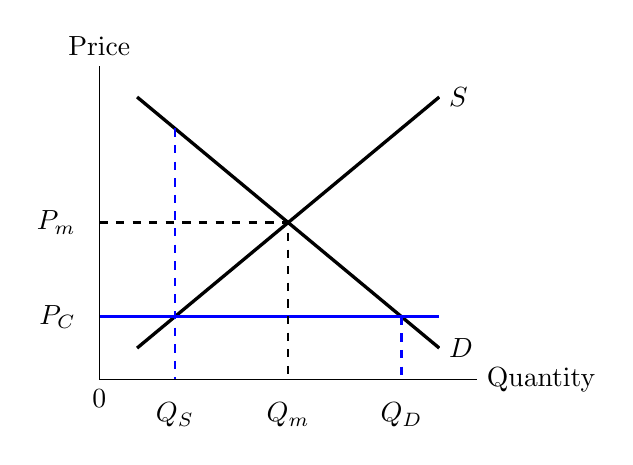
\begin{tikzpicture}
\begin{axis}[
scale=0.7,
xmin = 0, xmax = 10,
ymin = 0, ymax = 10, 
axis lines* = left,
xtick = {0}, ytick = \empty,
axis on top, 
clip = false,
]

\addplot[color = black, very thick] coordinates {(1,9) (9,1)};
\addplot[color = black, very thick] coordinates {(1,1) (9,9)};
\addplot[color = blue, very thick] coordinates {(0,2) (9,2)};

\addplot[color = black, dashed, thick] coordinates {(0,5) (5,5) (5,0)};
\addplot[color = blue, dashed, thick] coordinates {(2,8) (2,0)};
\addplot[color = blue, dashed, thick] coordinates {(8,2) (8,0)};

\node [right] at (current axis.right of origin) {Quantity};
\node [above] at (current axis.above origin) {Price};
\node [left = 5pt] at (0,5) {$P_m$};
\node [below = 5pt] at (5,0) {$Q_m$};
\node [right, fill = white] at (9,1) {$D$};
\node [right, fill = white] at (9,9) {$S$};
\node [below = 5pt] at (2,0) {$Q_S$};
\node [below = 5pt] at (8,0) {$Q_D$};
\node [left = 5pt] at (0,2) {$P_C$};
\end{axis}
\end{tikzpicture}
\caption{Market for NYC Apartments}
\label{fig:nycrentcontrol}
\end{center}
\end{figure}

Whats happening here is that the government has administered a price that is set \textbf{BELOW} the equilibrium price to prevent prices from rising to the equilibrium price. This example is easy to understand when looking at rent control in NYC apartments. Since the cost of living is so high in large cities like NYC, its difficult to house critical public employees with the wage they earn. So the government creates a ceiling, that prevents the price from exceeding a set amount. This causes a shortage, as demand is high but supply is low. $Q_S < Q_D$. The shortage cant resolve either, since it isnt able to increase to the equilibrium price.

Price ceilings end up creating inefficiencies in the market, and wasting resources. It costs extra to deal with the shortage, and means that some high value consumers cannot get it, while low value do get it. The quality of the good will also go down, as producers have no incentive to improve the quality. In the case of NYC apartments, the producer cannot raise prices to cover repairs. This also has the side effect of black market negotiations. 

\begin{figure}[H]
\begin{center}
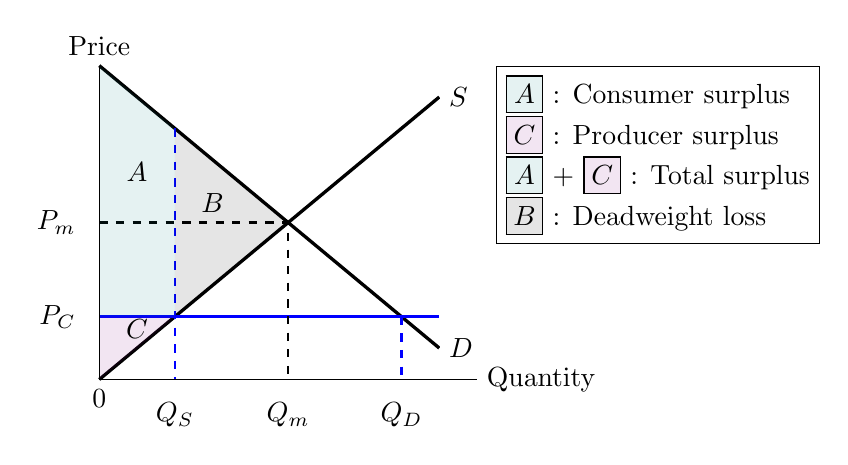
\begin{tikzpicture}
\begin{axis}[
scale=0.7,
xmin = 0, xmax = 10,
ymin = 0, ymax = 10, 
axis lines* = left,
xtick = {0}, ytick = \empty,
axis on top, 
clip = false,
]

\addplot[color = black, very thick] coordinates {(0,10) (9,1)};
\addplot[color = black, very thick] coordinates {(0,0) (9,9)};
\addplot[color = blue, very thick] coordinates {(0,2) (9,2)};

\addplot[color = black, dashed, thick] coordinates {(0,5) (5,5) (5,0)};
\addplot[color = blue, dashed, thick] coordinates {(2,8) (2,0)};
\addplot[color = blue, dashed, thick] coordinates {(8,2) (8,0)};

\fill[black, opacity = 0.1] (2,8) -- (5,5) -- (2,2);
\fill[teal, opacity = 0.1] (0,10) -- (2,8) -- (2,2) -- (0,2);
\fill[violet, opacity = 0.1] (0,0) -- (2,2) -- (0,2);

\node [above] at (1,6) {$A$};
\node [above] at (3,5) {$B$};
\node [above] at (1,1) {$C$};
\node [right] at (current axis.right of origin) {Quantity};
\node [above] at (current axis.above origin) {Price};
\node [left = 5pt] at (0,5) {$P_m$};
\node [below = 5pt] at (5,0) {$Q_m$};
\node [right, fill = white] at (9,1) {$D$};
\node [right, fill = white] at (9,9) {$S$};
\node [below = 5pt] at (2,0) {$Q_S$};
\node [below = 5pt] at (8,0) {$Q_D$};
\node [left = 5pt] at (0,2) {$P_C$};

\node [below right, draw, align = left] at (10.5, 10) {
\fcolorbox{black}{teal!10}{\makebox[\fontcharht\font`X]{$A$}} : Consumer surplus \\
\fcolorbox{black}{violet!10}{\makebox[\fontcharht\font`X]{$C$}} : Producer surplus \\
\fcolorbox{black}{teal!10}{\makebox[\fontcharht\font`X]{$A$}} + \fcolorbox{black}{violet!10}{\makebox[\fontcharht\font`X]{$C$}} : Total surplus \\
\fcolorbox{black}{black!10}{\makebox[\fontcharht\font`X]{$B$}} : Deadweight loss
};
\end{axis}
\end{tikzpicture}
\caption{Market for NYC Apartments}
\label{fig:nycrentcontrol2}
\end{center}
\end{figure}

This is the same graph, but highlights where specifically the DWL, the reduced PS and CS is. Since at $P_C: Q_D > Q_S$ a shortage exists. Producer surplus decreases, while consumer surplus does increase. TS decreases by DWL. Price ceilings make the market inefficient, but thats not the goal. They are used to make a market more equitable, rather than efficient. A ceiling can only operate if its placed \textbf{under} the equilibrium point. If its over, it becomes non-binding. 

Price floors on the other hand, do the opposite of a ceiling. The government administered a price that is set \textbf{ABOVE} the equilibrium price to prevent prices falling to the equilibrium price.

\begin{figure}[h!]
\begin{center}
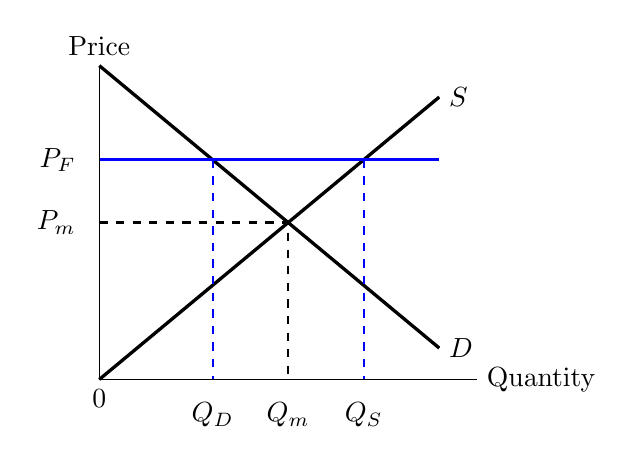
\begin{tikzpicture}
\begin{axis}[
scale=0.7,
xmin = 0, xmax = 10,
ymin = 0, ymax = 10, 
axis lines* = left,
xtick = {0}, ytick = \empty,
axis on top, 
clip = false,
]

\addplot[color = black, very thick] coordinates {(0,10) (9,1)};
\addplot[color = black, very thick] coordinates {(0,0) (9,9)};
\addplot[color = blue, very thick] coordinates {(0,7) (9,7)};

\addplot[color = black, dashed, thick] coordinates {(0,5) (5,5) (5,0)};
\addplot[color = blue, dashed, thick] coordinates {(3,7) (3,0)};
\addplot[color = blue, dashed, thick] coordinates {(7,7) (7,0)};

\node [right] at (current axis.right of origin) {Quantity};
\node [above] at (current axis.above origin) {Price};
\node [left = 5pt] at (0,5) {$P_m$};
\node [below = 5pt] at (5,0) {$Q_m$};
\node [right, fill = white] at (9,1) {$D$};
\node [right, fill = white] at (9,9) {$S$};
\node [below = 5pt] at (7,0) {$Q_S$};
\node [below = 5pt] at (3,0) {$Q_D$};
\node [left = 5pt] at (0,7) {$P_F$};
\end{axis}
\end{tikzpicture}
\caption{Market for Corn}
\label{fig:corn}
\end{center}
\end{figure}

An example where a price floor wouldbe useful is with agricultural products, as the industry has lobbied Congress to implement a price floor. Another example could be the minimum wage, when the cost of living becomes higher. With a price floor, a surplus exists, as $Q_D < Q_S$. The surplus cannot correct itself because of the floor. 

Price floors result in the same inefficiencies that price ceilings do, but in a different way. Instead of different consumer allocation, it focuses on producers. Some high cost producers can sell, while some low cost producers cannot. This causes wasted resources, and only benefits private industries. This also causes a sharp contrast in high quality and low quality goods, because of the DWL. Price floors are to help protect a particular industries or workers.

\begin{figure}[h!]
\begin{center}
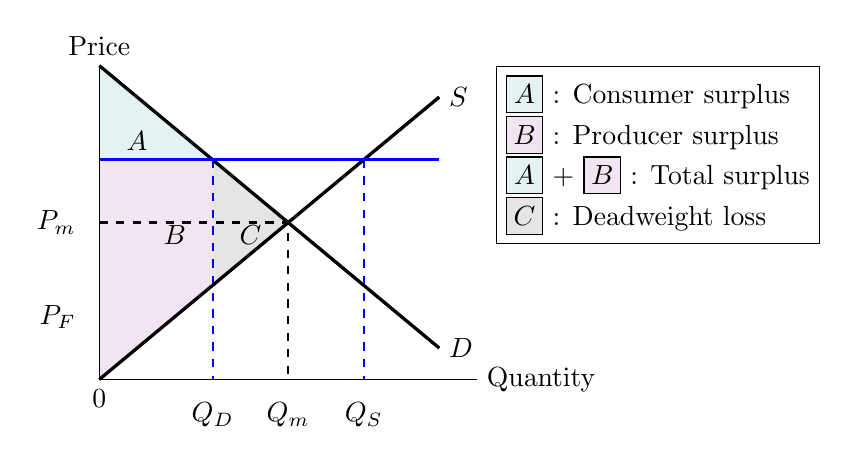
\begin{tikzpicture}
\begin{axis}[
scale=0.7,
xmin = 0, xmax = 10,
ymin = 0, ymax = 10, 
axis lines* = left,
xtick = {0}, ytick = \empty,
axis on top, 
clip = false,
]

\addplot[color = black, very thick] coordinates {(0,10) (9,1)};
\addplot[color = black, very thick] coordinates {(0,0) (9,9)};
\addplot[color = blue, very thick] coordinates {(0,7) (9,7)};

\addplot[color = black, dashed, thick] coordinates {(0,5) (5,5) (5,0)};
\addplot[color = blue, dashed, thick] coordinates {(3,7) (3,0)};
\addplot[color = blue, dashed, thick] coordinates {(7,7) (7,0)};

\fill[teal, opacity = 0.1] (0,10) -- (3,7) -- (0,7);
\fill[black, opacity = 0.1] (3,7) -- (5,5) -- (3,3);
\fill[violet, opacity = 0.1] (0,7) -- (3,7) -- (3,3) -- (0,0);

\node [below right, draw, align = left] at (10.5, 10) {
\fcolorbox{black}{teal!10}{\makebox[\fontcharht\font`X]{$A$}} : Consumer surplus \\
\fcolorbox{black}{violet!10}{\makebox[\fontcharht\font`X]{$B$}} : Producer surplus \\
\fcolorbox{black}{teal!10}{\makebox[\fontcharht\font`X]{$A$}} + \fcolorbox{black}{violet!10}{\makebox[\fontcharht\font`X]{$B$}} : Total surplus \\
\fcolorbox{black}{black!10}{\makebox[\fontcharht\font`X]{$C$}} : Deadweight loss
};

\node [above] at (1,7) {$A$};
\node [above] at (2,4) {$B$};
\node [above] at (4,4) {$C$};
\node [right] at (current axis.right of origin) {Quantity};
\node [above] at (current axis.above origin) {Price};
\node [left = 5pt] at (0,5) {$P_m$};
\node [below = 5pt] at (5,0) {$Q_m$};
\node [right, fill = white] at (9,1) {$D$};
\node [right, fill = white] at (9,9) {$S$};
\node [below = 5pt] at (7,0) {$Q_S$};
\node [below = 5pt] at (3,0) {$Q_D$};
\node [left = 5pt] at (0,2) {$P_F$};
\end{axis}
\end{tikzpicture}
\caption{Market for NYC Apartments}
\label{fig:nycrentcontrol}
\end{center}
\end{figure}

Since at minimum wage, $Q_S > Q_D$, there is a surplus of workers. CS goes down, while producer surplus goes up. Total surplus is still reduced by DWL. The floor in this scenario increase unemployment. Some will lose their job, and can only calculate if exact numbers are given. For a price floor to be binding, it must be placed \textbf{above} the equilibrium point. If its placed below, it becomes non-binding.

